\chapter{Objektsysteme in Racket}
Racket ist ein Dialekt von Lisp, der auf Scheme basiert\cite{racketguide-dialects}. Es ist jedoch keine rein funktionale Sprache, sondern unterstützt verschiedene Lisp-Dialekte und  Programmierparadigmen. 
%Damit gibt Racket Programmierern und Forschern die Werkzeuge, die sie benötigen, um neue Sprachen zu erkunden und zu entwickeln\cite{racketguide-dialects} und wird beispielsweise auch an der Universität Hamburg in der Forschung genutzt.

Racket wird in der Softwareentwicklungslehre genutzt, da es im Gegensatz zu Common Lisp sehr einsteigerfreundlich ist. Die Veranstaltungsteilnehmer lernen zum ersten Mal eine funktionale Sprache kennen und sollen einen möglichst einfachen Einstieg erhalten. Hierzu bietet Racket eine übersichtliche Syntax und eine plattformunabhängige Entwicklungsumgebung, die vergleichbare Fehlermeldungen liefert.

In Common Lisp wird die Syntax schnell sehr komplex und ist zudem abhängig von der Implementierung (teilweise sogar mit kostenpflichtigem Interpreter). Common Lisp hat zwei verschiedene Paketsysteme mit tausenden von Paketen, was ein schnelles Zurechtfinden in der Sprache nicht unbedingt begünstigt. Es gibt keine dedizierte grafische Oberfläche, da Common Lisp für die Integration in Emacs, Vim etc. ausgelegt ist. Das würde bedeuten, dass Veranstaltungsteilnehmer sich erst einmal mit der Integration der Sprache in den Editor ihrer Wahl beschäftigen müssten, bevor sie überhaupt eine Zeile Code schreiben können. Nicht alle Interpreter von Common Lisp werden auch für alle Betriebssysteme gewartet, wie zum Beispiel SBCL, der zwar frei und gut ist, aber unter Windows nur gelegentlich gepflegt wird. Das macht es extrem schwer die Ursache von Fehlern zu erkennen, da immer auch das Betriebssystem bedacht werden muss. Zudem ist eine systemübergreifende grafische Ausgabe ohne weitere Pakete nicht vorgesehen. Das erschwert das Stellen von Aufgaben, bei denen das Ergebnis visualisiert werden kann oder muss, da die grafische Ausgabe vom Interpreter abhängig ist und die Teilnehmer zudem erst einmal die entprechenden Pakete installieren müssten. 

Um Common Lisp zu lernen, wurde daher Scheme entwickelt. Analog zu BlueJ, einer Entwicklungsumgebung für das Lernen von objektorientierter Programmierung in Java, war DrScheme das Einsteigertool zu Common Lisp. Im Jahr 2010 wurde Scheme umbenannt zu Racket. Racket bildet einen guten Kompromiss für die Lehre, da es einen einfachen Einstieg in die Welt von Common Lisp bietet.
%----------------------

Die Syntax von Racket ist sehr ähnlich zu Common Lisp. Ausdrücke werden geklammert, Kommentare mit einem Semikolon eingeleitet. Einige Standardfunktionen haben leicht abgewandelte Namen. So werden in Racket beispielsweise sowohl Funktionen als auch Variablen mit dem Schlüsselwort \texttt{define} definiert, anstelle von \texttt{defun}, \texttt{defvar} und \texttt{defparameter} in Common Lisp. Prädikate enden auf \texttt{?} (zum Beispiel \texttt{equal?}) und Methoden, die Variablen oder Objekte verändern auf \texttt{!} (zum Beispiel \texttt{set!}). Einer der größeren Unterschiede liegt in der Art, wie Makros definiert werden; darauf wird im Kapitel \ref{makros} noch näher eingegangen.

Racket unterstützt auch objektorientierte Programmierung auf zwei verschiedene Arten. Zunächst gibt das Racket-Objektsystem. Racket-Klassen sind sehr ähnlich zu Klassen in Java, C\# oder den meisten objektorientierten Programmiersprachen\cite{neu-edu2}. Ein Programm kann Klassen definieren, instanziieren, mit den erzeugten Objekten interagieren und Klassen erweitern. Besonders ist, dass Klassen auch wie Funktionswerte behandelt werden können. Es ist möglich, eine Klasse zur Laufzeit zu erweitern, eine Klasse an eine Funktion zu geben oder in einer Datenstruktur zu speichern und anschließend abzufragen\cite{neu-edu}. 

Zusätzlich gibt es den Racket-Dialekt Swindle, in dem das Common Lisp Object System (CLOS) implementiert ist. Im Gegensatz zum eingebauten Objektsystem von Racket bietet CLOS Funktionalitäten wie Mehrfachvererbung, Methodenkombination oder Ergänzungsmethoden. Durch die Implementation als Metaobject-Protocol bietet es dem Programmierer zudem viel Freiheit bei der Erweiterung und Veränderung der Repräsentation von Klassen und Objekten.
Um ein Gefühl für die beiden Objektsysteme zu bekommen, soll zunächst betrachtet werden, wie sie benutzt werden können. %Andschließend wird ein Blick auf die Implementation beider Ansätze geworfen. Die Autoren des Buches ``The Art of the Metaobject Protocol''\cite{amop} vergleichen das Vorgehen sehr treffend mit eine Theateraufführung: Auf der Bühne (onstage) findet das Theaterstück statt - das Programm, oder etwas allgemeiner, das, was der Programmierer von der Sprache sieht. Hinter der Bühne (backstage) befindet sich die darunterliegende Implementation, die die entprechenden Makros definiert und mit für den Programmierer nicht sichtbaren Objekten und Funktionen arbeitet. Wir wollen beide Ansätze erst ``onstage'' betrachten bevor wir einen Blick hinter die Kulissen werfen.

Der Fokus dieser Arbeit liegt auf der Implementation von Mehrfachvererbung im Objektsystem von Racket. Natürlich bieten sowohl das Objektsystem von Racket als auch CLOS neben Vererbung auch noch viele weitere nützliche Funktionen und Eigenschaften; diese sind jedoch nicht zielführend für diese Arbeit und es würde eine eigene Ausarbeitung benötigen, sie alle aufzulisten. Im Folgenden wird daher nur auf diejenigen Bestandteile beider Ansätze eingegangen, die direkt oder indirekt mit Mehrfachvererbung zu tun haben. 

Die Installation von Racket beinhaltet eine integrierte Enwicklungsumgebung namens DrRacket. Für das Syntaxhighlighting der Quelltextbeispiele in dieser Arbeit wurde das Standard-Farbschema von DrRacket verwendet. Anfragen an die Interaktionskonsole wurden mit \texttt{>} markiert und das Ergebnis in der Zeile darunter aufgeführt. 

\section{Beispielproblem} 

%TODO Beispielproblem überarbeiten 

Beide Objektsysteme sollen anhand eines Beispielproblems beschrieben werden. Es soll zunächst das Verhalten einfacher Klassen und Einfachvererbung gezeigt werden und darauf aufbauend die Konzepte von Mehrfachvererbung, die in den Objektsystemen vorhanden sind. Ziel wird es daher sein, die folgende Vererbungshierarchie zu implementieren:

\begin{figure}[h]
 \centering
 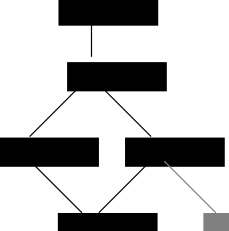
\includegraphics[width=0.35\textwidth]{pictures/hirarchy}
 \caption{Vererbungshierarchie für die Klasse Pokemon.}
 \label{hirarchy}
\end{figure}

Die Klasse Thing soll eine einfache Basisklasse sein und uns die Möglichkeit geben, die Syntax der Klassendefinition beider Ansätze zu vergleichen. Da Thing ledigleich eine leere Klasse ist, wollen wir im Anschluss zwei Klassen erstellen, deren Felder und Methoden später vererbt werden können: Element und Animal. Anhand von Element betrachten wir dabei zunächst, wie Felder und Methoden definiert werden können. Anhand der Klasse Animal und ihrer Subklasse Pet können wir das Konzept der Vererbung veranschaulichen. Es wird dann mit der Klasse Pokemon gezeigt, welche Möglichkeiten der Mehrfachvererbung es gibt.

Zusätzlich soll für beide Objektsysteme geprüft werden, welche Möglichkeiten es gibt, Methoden einer Superklasse in einer Subklasse zu ergänzen. 